\documentclass[11pt,a4paper]{article}

% --- Essential Packages ---
\usepackage[utf8]{inputenc}
\usepackage[a4paper, margin=0.75in]{geometry}
\usepackage{mathptmx}
\usepackage{amsmath,amssymb}
\usepackage{graphicx}
\usepackage{booktabs}
\usepackage{xcolor}
\usepackage{colortbl}
\usepackage{hyperref}
\usepackage{float}
\usepackage{tikz}
\usepackage{eso-pic}
\usepackage{parskip}

% --- Light Thin Border on All Pages ---
\AddToShipoutPictureBG{%
  \begin{tikzpicture}[remember picture, overlay]
    \draw[line width=0.6pt, color=gray!50]
      ([shift={(10mm,-10mm)}]current page.north west)
      rectangle
      ([shift={(-10mm,10mm)}]current page.south east);
  \end{tikzpicture}%
}

% --- Hyperlink Setup ---
\hypersetup{
    colorlinks=true,
    linkcolor=blue!70!black,
    citecolor=blue!70!black,
    urlcolor=blue!70!black
}

\begin{document}

% --- Header Block ---
\begin{center}
    {\LARGE \textbf{Minimal Gene Signature Discovery - Report}}\\[0.6em]
    \textbf{Team:} 5 - \textbf{Batch:} AIDM-A\\[1.0em]
    
    {\renewcommand{\arraystretch}{1.35}%
    \setlength{\tabcolsep}{18pt}%
    \arrayrulecolor{gray!50}%
    \begin{tabular}{|c|c|}
        \hline
        \multicolumn{2}{|c|}{\textbf{Team Members}} \\
        \hline
        Anuragine S A & CB.AI.U4AIM24005 \\
        \hline
        Naresh L & CB.AI.U4AIM24028 \\
        \hline
        Ragul U & CB.AI.U4AIM24036 \\
        \hline
    \end{tabular}}
\end{center}
\vspace{1.8em}
\hrule
\vspace{1.0em}

\section{Addressing Class Imbalance in Dataset}

The dataset used in this work is GSE2034, which contains 286 breast cancer patients. In this dataset:
\begin{itemize}
    \item 217 patients did not have their cancer return (non-relapse, 75.9\%).
    \item 69 patients had their cancer return (relapse, 24.1\%).
\end{itemize}
We split the 286 patients into two groups: 80\% for training and 20\% for testing. 
\begin{itemize}
    \item \textbf{Training set (228 patients):} 173 non-relapse and 55 relapse patients.
    \item \textbf{Test set (58 patients):} 44 non-relapse and 14 relapse patients.
\end{itemize}
All models were trained on the training set and tested on the test set using the 5 selected genes: \textit{SLC35E3}, \textit{NTM}, \textit{RECQL4}, \textit{TNFRSF10C}, and \textit{CPB1}.

\subsection{Problem Caused by Imbalance}
There are roughly three times more non-relapse patients than relapse patients. Because of this, a regular model tries to get a good overall score by mostly predicting the majority class (non-relapse).

When we train a standard Logistic Regression model without adjusting for this:
\begin{itemize}
    \item The model looks like it is working well because overall accuracy is 72.4\%, and specificity (correctly finding non-relapse patients) is 90.9\% (40 out of 44).
    \item But for the relapse patients, the model correctly identifies only 2 out of the 14 relapse patients. That is a sensitivity of only 14.3\%. It misses 12 out of 14 patients whose cancer returned.
\end{itemize}
In medical prediction, missing patients whose cancer returns is a serious problem. Even though the overall ROC-AUC score is 0.679, the standard model misses most of the high-risk patients because the decision cutoff is not adjusted for the unequal group sizes.

\subsection{Our Fix for Imbalance}
To fix this, we used balanced class weighting (\texttt{class\_weight='balanced'} in scikit-learn). 

Normally, the model gets the same penalty for any mistake. With balanced weighting, we tell the model that making a mistake on a rare relapse patient is worse than making a mistake on a common non-relapse patient. The weight for each class is calculated using this simple formula:
\begin{equation}
\text{Weight} = \frac{\text{Total Training Patients}}{2 \times \text{Patients in that Group}}
\end{equation}
For our training set of 228 patients:
\begin{equation}
\text{Weight for Non-Relapse} = \frac{228}{2 \times 173} = 0.66, \qquad 
\text{Weight for Relapse} = \frac{228}{2 \times 55} = 2.07
\end{equation}
Because 2.07 is about 3.14 times larger than 0.66, the model receives a penalty that is 3.14 times higher when it misses a relapse patient.

\subsection{Results After Adding Balanced Weights}
When we test the balanced Logistic Regression model on the 58 test patients:
\begin{itemize}
    \item \textbf{Relapse Sensitivity:} The model now catches 9 out of the 14 relapse patients (64.3\% sensitivity), compared to only 2 out of 14 before (14.3\%).
    \item \textbf{Balanced Accuracy:} Balanced accuracy is the average of sensitivity and specificity. It goes up from 52.6\% to 62.8\%.
    \item \textbf{ROC-AUC:} The ROC-AUC stays almost identical at 0.674 (compared to 0.679 for unweighted).
    \item \textbf{Precision-Recall AUC (PR-AUC):} The PR-AUC is 0.401. If a model was just guessing randomly, the PR-AUC would be 0.241 (the proportion of relapse patients, 14/58). Reaching 0.401 shows that the model is using genuine signal from the 5 genes.
\end{itemize}

\section{Comparison with K-Nearest Neighbors (KNN)}

We also tested K-Nearest Neighbors (KNN, with $k=5$) on the exact same 5 genes.

\subsection{How KNN Works}
KNN is a distance-based method. In our implementation:
\begin{enumerate}
    \item To predict the outcome for a new test patient, it looks at that patient's expression values for the 5 genes.
    \item It measures the straight-line distance (Euclidean distance) between this patient and every patient in the training set.
    \item It finds the 5 closest training patients.
    \item It checks what happened to those 5 neighbors. If most of them had a relapse, it predicts relapse. If most of them did not, it predicts non-relapse.
\end{enumerate}

\subsection{Test Results for KNN}
When evaluated on the 58 test patients:
\begin{itemize}
    \item \textbf{ROC-AUC:} KNN achieves an ROC-AUC of 0.630, which is lower than Logistic Regression (0.674).
    \item \textbf{Relapse Sensitivity:} KNN correctly catches only 3 out of 14 relapse patients (21.4\% sensitivity), missing 11 relapse patients.
    \item \textbf{Balanced Accuracy:} KNN gets 56.2\%, which is lower than balanced Logistic Regression (62.8\%).
\end{itemize}

\subsection{Why Logistic Regression Performs Better Than KNN}
There are two main reasons why Logistic Regression performs better on this data:
\begin{enumerate}
    \item \textbf{Noise in gene data:} Microarray gene expression measurements have natural biological noise. Because KNN only looks at the 5 closest individual patients, even a small amount of measurement noise can change which patients end up as the closest neighbors. In contrast, Logistic Regression looks at all 228 training patients together to find one general trend, so it is less affected by individual noisy points.
    \item \textbf{Class imbalance in the neighborhood:} Because 76\% of the training patients are non-relapse, most regions in the data have more non-relapse patients. This makes it difficult for a test patient to have a majority of relapse neighbors in KNN.
\end{enumerate}

\section{Summary of Results}

The table below summarizes the test performance for each model on the 58 test patients:

\begin{table}[H]
\centering
\resizebox{\textwidth}{!}{%
\begin{tabular}{lccccccc}
\toprule
\textbf{Model} & \textbf{ROC-AUC} & \textbf{PR-AUC} & \textbf{Balanced Acc.} & \textbf{Sensitivity} & \textbf{Specificity} & \textbf{Relapses Caught} & \textbf{No-Relapses Caught} \\
\midrule
Logistic Regression (Unweighted) & 0.679 & 0.404 & 52.6\% & 14.3\% & 90.9\% & 2 / 14 & 40 / 44 \\
Logistic Regression (Balanced)   & 0.674 & 0.401 & 62.8\% & 64.3\% & 61.4\% & 9 / 14 & 27 / 44 \\
K-Nearest Neighbors (KNN, $k=5$) & 0.630 & 0.374 & 56.2\% & 21.4\% & 90.9\% & 3 / 14 & 40 / 44 \\
\bottomrule
\end{tabular}%
}
\end{table}

The bar charts below show the comparison of ROC-AUC, Balanced Accuracy, and relapse detection sensitivity:

\begin{figure}[H]
\centering
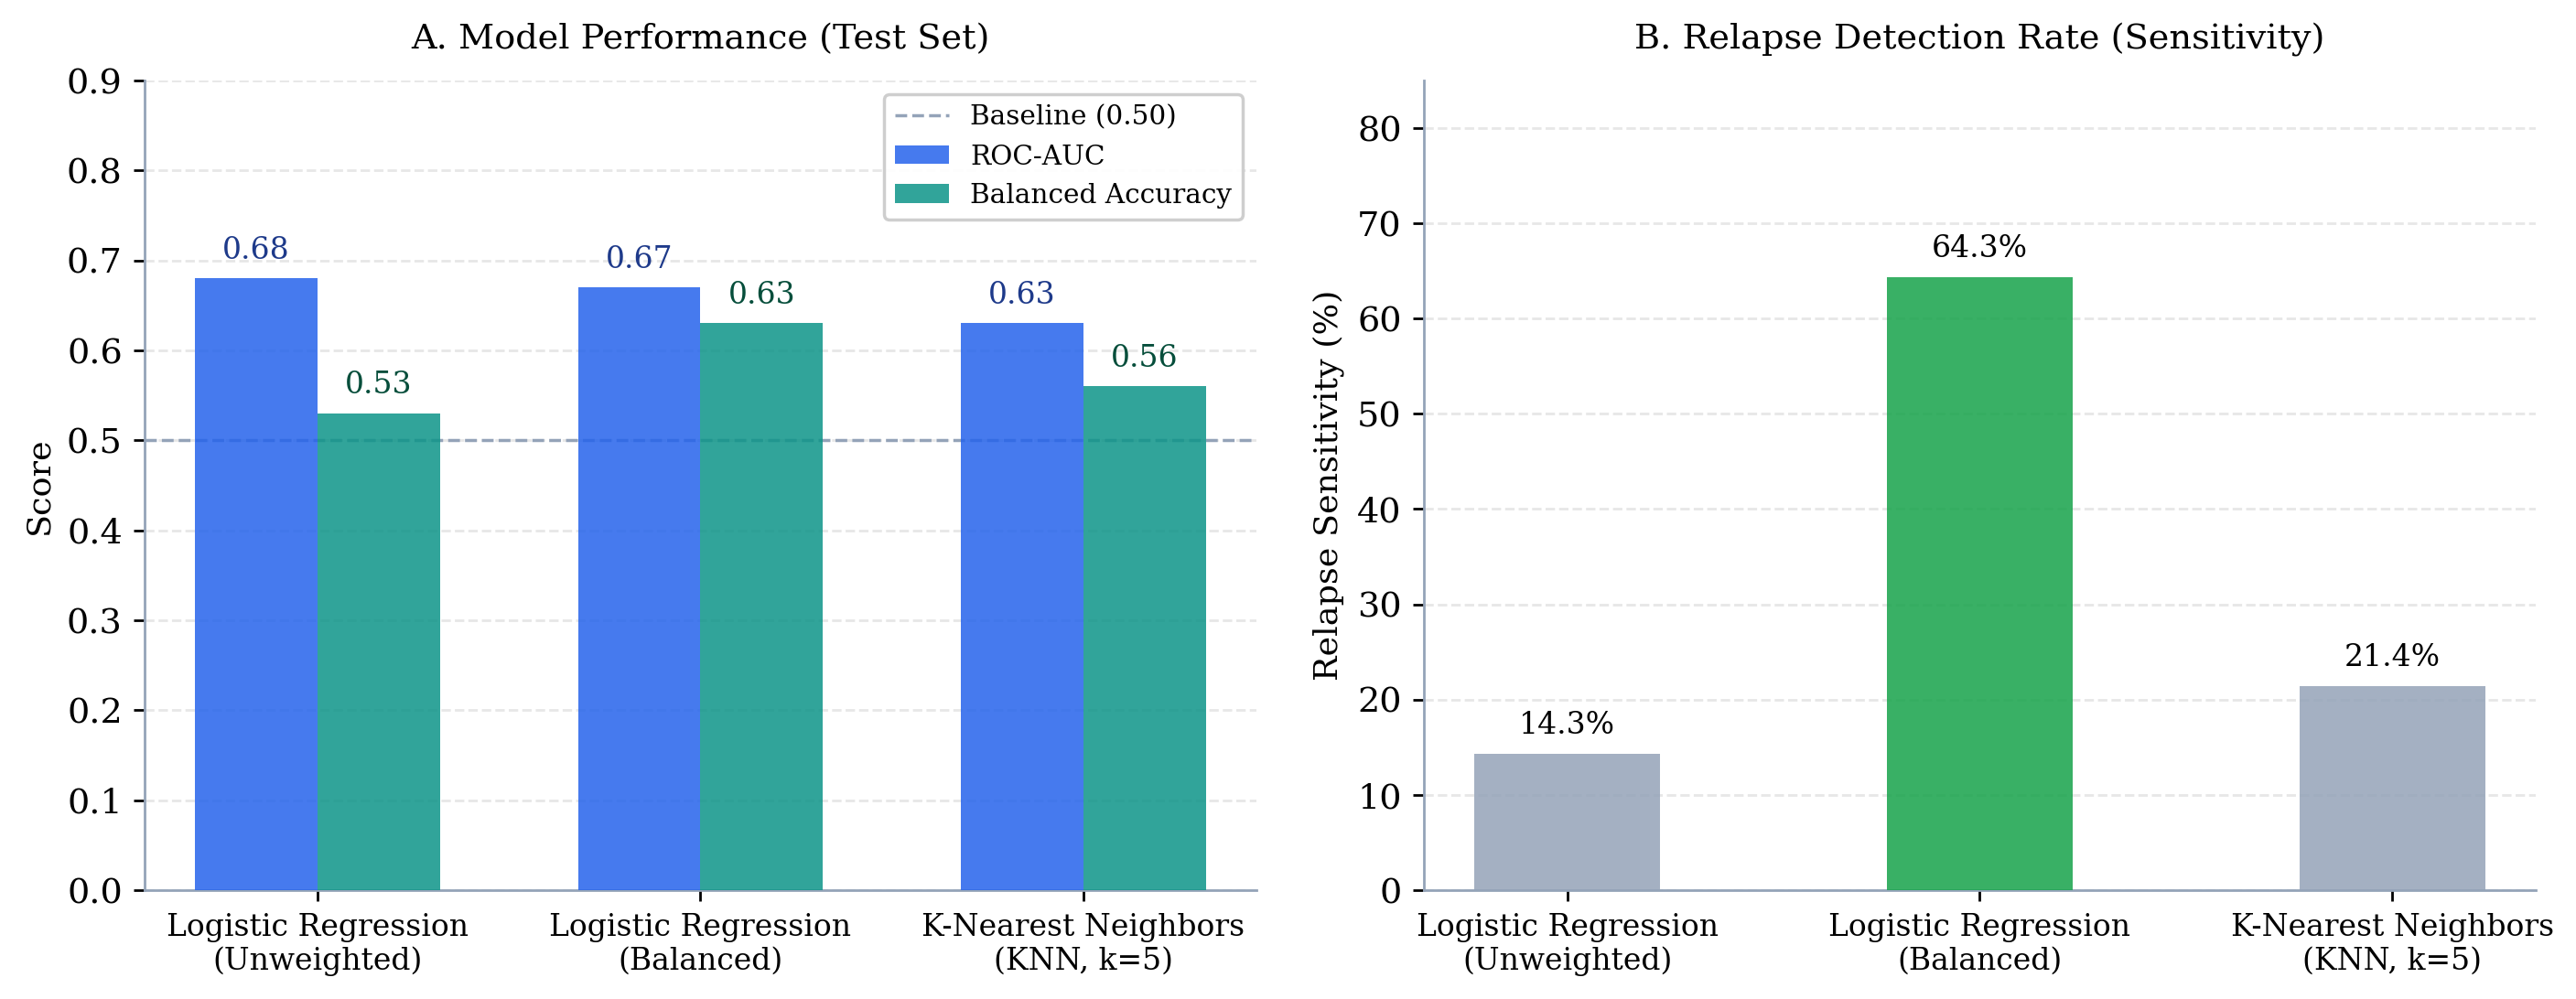
\includegraphics[width=\textwidth]{report_figure.png}
\end{figure}

\section{Conclusion}

These are our inferences from this experiment:
\begin{enumerate}
    \item \textbf{Class Imbalance:} When 76\% of patients do not have a relapse, a standard unweighted model misses most relapse patients (only catching 2 of 14). Adding balanced weights fixes this by penalizing missed relapse cases more heavily. This increases relapse detection to 9 of 14 (64.3\% sensitivity) and improves balanced accuracy to 62.8\%.
    \item \textbf{Comparison with KNN:} Logistic Regression works better than KNN on this dataset (0.674 vs 0.630 ROC-AUC, and 64.3\% vs 21.4\% sensitivity). Logistic Regression finds a single general trend across all 228 training patients, whereas KNN relies on local distances between individual patients that are more easily affected by noise.
\end{enumerate}

\end{document}
